% !TEX TS-program = xelatex
% !TEX encoding = UTF-8 Unicode

% \documentclass[AutoFakeBold]{LZUThesis}
\documentclass[AutoFakeBold]{LZUThesis}
\usepackage{float}
\begin{document}
%=====%
%
%封皮页填写内容
%
%=====%

% 标题样式 使用 \title{{}}; 使用时必须保证至少两个外侧括号
%  如: 短标题 \title{{第一行}},  
% 	      长标题 \title{{第一行}{第二行}}
%             超长标题\tiitle{{第一行}{...}{第N行}}

\title{{基于深度学习的乳腺癌检测}}



% 标题样式 使用 \entitle{{}}; 使用时必须保证至少两个外侧括号
%  如: 短标题 \entitle{{First row}},  
% 	      长标题 \entitle{{First row}{ Second row}}
%             超长标题\entitle{{First row}{...}{ Next N row}}
% 注意:  英文标题多行时 需要在开头加个空格 防止摘要标题处英语单词粘连。
\entitle{{Breast cancer detection based on deep learning}}

\author{姚忱}
\major{电子信息科学与技术}
\advisor{张红娟}
\college{信息科学与工程学院}
\grade{2019级}



\maketitle

%==============================%
% ↓ ↓ ↓ 诚信说明页 授权说明书
%==============================%

% 1. 可以调整签字的宽度,现在是40
% 2. 去掉raisebox的相关注释(注意上下大括号对应),可以改变-5那个数字调整签名和横线的上下位置

% 你的签名,signature.pdf 改为你的签名文件名,
%\mysignature{
    % \raisebox{-5pt}{
       % 
\includegraphics[width=40pt]{signature.pdf}
    % }
%  }
% 你手写的日期,signature.pdf 改为你的手写的日期文件名
%\mytime{
    % \raisebox{-5pt}{
        %
\includegraphics[width=40pt]{signature.pdf}
    % }
%}
% 老师的手写签名,signature.pdf 改为老师的手写签名文件名
%\supervisorsignature{
    % \raisebox{-5pt}{
        %
\includegraphics[width=40pt]{signature.pdf}
    % }
%}
% 老师手写的时间,signature.pdf 改为老师的手写的日期文件名
%\teachertime{
    % \raisebox{-5pSt}{
       % 
\includegraphics[width=40pt]{signature.pdf}
    % }
%}
% 老师手写的成绩
%\recommendedgrade{
    % \raisebox{-5pt}{
       % 
\includegraphics[width=40pt]{signature.pdf}
    % }
%}

\makestatement

%==============================%
% ↑ ↑ ↑ 诚信说明页 授权说明书
%==============================%


%=====%
%论文(设计)成绩:注意2007的模板要求,成绩页在最后,2021要求成绩页在摘要前面
%=====%

% 下面这些注释掉可以去掉成绩、评语什么的
\supervisorcomment{导师评价你人很好}


\committeecomment{优秀}

\finalgrade{100}
% 上面这些注释掉可以去掉成绩、评语什么的


\frontmatter



%中文摘要
\ZhAbstract{本项目使用了深度学习技术来实现乳腺癌的早期诊断。项目是在INbreast,BraeakHis等乳腺癌图像数据集上训练CNN模型来对乳腺癌病例进行分类。比较了不同的数据集,不同的CNN模型及不同的分类方式的表现,并在验证集上使用准确度等指标评估模型的性能。最终,项目提供了一个使用Keras实现的CNN模型,该模型可以准确地分类乳腺癌图像}{乳腺癌,深度学习,卷积神经网络}


%英文摘要
\EnAbstract{This project uses deep learning technology to achieve early diagnosis of breast cancer. The project is to train a CNN model on INbreast, BraeakHis and other breast cancer image datasets to classify breast cancer cases. The performance of different datasets, different CNN models and different classification methods is compared, and the performance of the model is evaluated using indicators such as accuracy on the verification set. Ultimately, the project provides a CNN model implemented using Keras that can accurately classify breast cancer images.\fontspec{Times New Roman}}
{Breast Cancer;Deep Learing;Convolutional Neural Network}

%生成目录
% \tableofcontents
% 下面这个包含图表目录
\customcontent


% % 部分同学需要专业术语注释表,* 表示不加入目录
% \chapter*{专业术语注释表}
% \begin{longtable}{lll}
%   \caption*{缩略词说明}\\
%   SS & Spread Spectrum & 扩展频谱 \\
%   PAPR & Peak to Average Power Ratio & 峰均比\\
%   DCSK & Differential Chaos Shift Keying &差分混移位键控\\   
%   dasd & fdhfudw eqwrqw fasfasfs fewev wqfwefew &\tabincell{l}{太长了\\换行一下}\\
% \end{longtable}


%文章主体
\mainmatter

\chapter{绪 \qquad 论}

% !学校要求的规范,绪论是单独的,不是第一章,但是老师们都是让作为第一章,这里我把它放在了论文里,如果你要让在外面,只需要把上面的 \mainmatter 这一句话放在“绪论内容后面,正文第一章前面”即可,也就是 \chapter{latex部分用法简介} 这一句话上面


\section{问题背景及研究意义}

乳腺癌是全球女性最为常见的恶性肿瘤之一。据国家癌症中心最新统计,全国每年新发乳腺癌病例数达27.24万,死亡人数超过7万。
其发病率呈现明显的上升趋势,高居女性恶性肿瘤发病率首位,已经成为女性健康的巨大威胁。
自上世纪八十年代以来,乳腺癌在中国的发病率持续快速上升,并呈现年轻化趋势,这对女性健康造成了严重的威胁。
早期发现和诊断乳腺癌是治愈该病的关键,因此乳腺癌检测技术备受瞩目。

然而,传统的乳腺癌检测技术,如组织病理学检查,乳房X线摄影和超声波检查等,存在着诸多限制,如良恶性病变的区分困难和漏诊率高等问题。
随着深度学习技术的不断发展,越来越多的学者开始研究基于深度学习的乳腺癌检测技术,以期改善传统技术所存在的局限性。



\chapter{基本原理与方法介绍}
\section{研究方法}
乳腺癌的诊断一直依赖于传统的组织病理学检查。然而,病理学家对组织图像进行人工分析是一项耗时且繁琐的过程,其诊断结果存在较大的主观性和误差风险。

因此,本研究旨在利用深度卷积神经网络(CNN)模型对乳腺癌图像进行分类,以提高乳腺癌诊断的准确性和效率。
我们使用不同的乳腺癌图像数据集来训练CNN模型,并对分类结果进行比较分析。

\section{卷积神经网络简介}
卷积神经网络(Convolutional Neural Network,CNN)是一种广泛应用于计算机视觉领域的人工神经网络模型。
CNN的基本思想是将输入图像作为网络的输入,并通过一系列卷积层、池化层、全连接层、非线性激活函数等操作,提取出图像的特征并进行分类或识别等任务。
CNN的主要优点是它可以自动学习输入数据的特征,从而无需手动设计特征提取器,因此被广泛应用于图像识别、目标检测、人脸识别、自然语言处理等各个领域。

\begin{figure}[H]
    \centering
    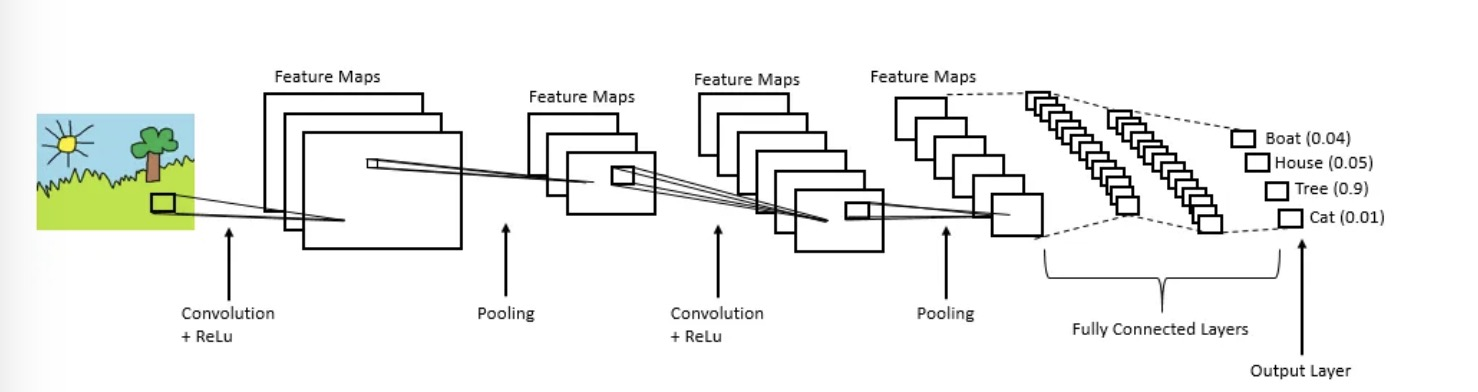
\includegraphics[scale=0.2]{4.jpeg}
    \caption{CNN基本结构}
    \label{figure}
 \end{figure}

\section{卷积神经网络基本结构}
\subsection{卷积层}

卷积神经网络(Convolutional Neural Network,CNN)中的卷积层是其核心部分之一。卷积层通过卷积运算对输入进行特征提取,并生成输出特征图。每个卷积层通常由多个过滤器(也称为卷积核)组成,每个过滤器都是一个小的可学习的权重矩阵,用于在输入上进行卷积运算,从而提取出局部特征。卷积运算通常会对输入的每个像素及其周围的像素进行权重相乘和加和的操作,从而生成一个新的特征图,该特征图对输入的局部区域进行了下采样和特征提取,且保留了局部位置信息。

在CNN中,每个卷积层的过滤器数量和大小通常是预先设定的,而过滤器的权重则通过反向传播算法进行训练。在训练过程中,CNN会通过反向传播来调整过滤器的权重,以最小化输出特征图与标签之间的差距。通过反复的训练,CNN可以逐渐优化卷积层的过滤器,使其能够提取出更加抽象和高级的特征,从而提高模型的性能和泛化能力。

卷积层的计算公式可以表示为:

$$
y_{i,j} = \sum_{m=0}^{k-1} \sum_{n=0}^{k-1} x_{i+m, j+n} \cdot w_{m, n} + b
$$

其中,$x$ 表示输入特征图,$y$ 表示输出特征图,$w$ 表示卷积核权重矩阵,$b$ 表示偏置项,$k$ 表示卷积核的大小。

具体来说,对于输出特征图中的每一个像素点 $(i,j)$,我们会将该像素点周围的 $k \times k$ 个像素点与卷积核中的权重矩阵进行卷积操作,即对于卷积核中的每一个权重 $w_{m,n}$,将输入特征图中位置为 $(i+m, j+n)$ 的像素点乘以该权重,然后将所有乘积加起来,并加上偏置项 $b$,即为该像素点在输出特征图中的值 $y_{i,j}$。
这个过程可以看做是对输入特征图进行局部的线性变换和下采样,从而提取出输入特征图的局部特征。实现如下图所示:

\begin{figure}[H]
    \centering
    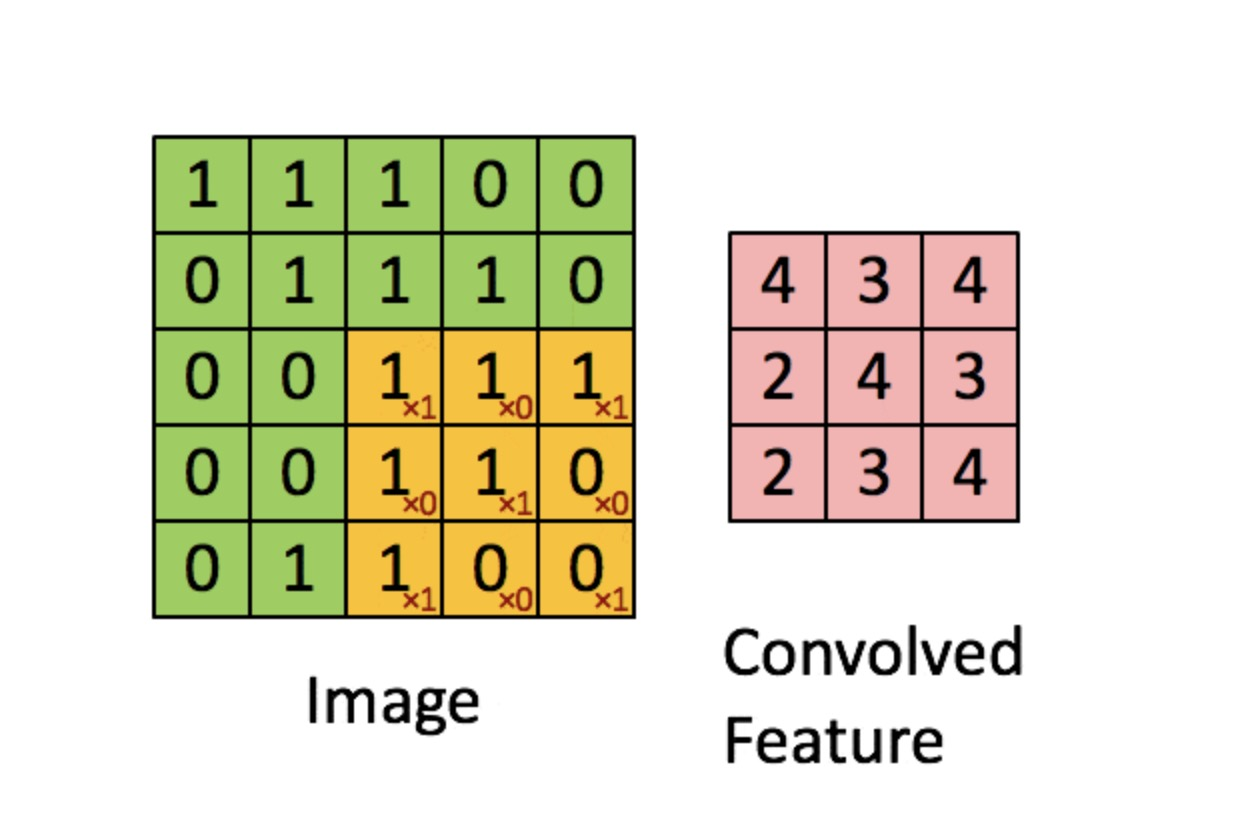
\includegraphics[scale=0.2]{5.jpeg}
    \caption{卷积层实现}
    \label{figure}
 \end{figure}

\subsection{池化层}
池化层是卷积神经网络中一种常用的层次结构,

池化操作通常分为最大池化和平均池化两种,其中最大池化是取输入特征图中每个子区域的最大值,
而平均池化是取每个子区域的平均值。池化操作的参数通常由池化窗口大小和步幅大小两个参数决定。
池化窗口大小指的是取样区域的大小,而步幅大小指的是池化窗口在特征图上移动的距离。

池化层的作用是降低特征图的维度,减少计算量和模型参数数量,从而防止过拟合。
池化层可以对每个卷积核提取的特征图进行下采样操作,从而在保留特征信息的同时,将特征图的尺寸降低一定程度上,
增强模型的泛化能力。



最大池化的计算公式为:
$$y_{i,j} = \max_{m,n}(x_{(i-1)s+m,(j-1)s+n})$$
其中,$x$是输入特征图,$y$是输出特征图,$s$是池化窗口的步幅大小,$m$和$n$是池化窗口内的像素坐标。

平均池化的计算公式为:
$$y_{i,j} = \frac{1}{k^2}\sum_{m=1}^k\sum_{n=1}^k x_{(i-1)s+m,(j-1)s+n}$$
其中,$k$是池化窗口的大小。

以最大池化为例,实现过程如下图:
\begin{figure}[H]
    \centering
    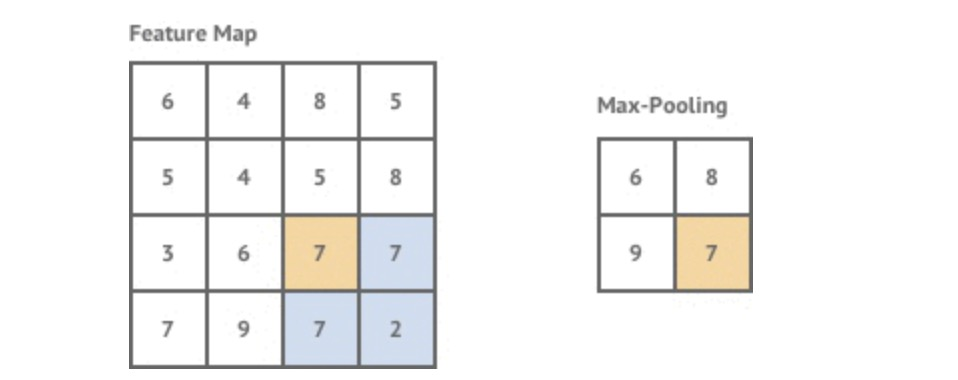
\includegraphics[scale=0.2]{6.jpeg}
    \caption{池化层实现}
    \label{figure}
 \end{figure}

\subsection{全连接层}
在卷积神经网络中,全连接层是一种用于对特征进行分类或者回归的层次结构。
全连接层接收前面所有层次的输出,将其展开为一个一维向量,并将其与一组权重进行乘积和偏置相加,最终输出一个新的向量,用于进行分类或回归任务。

在卷积神经网络的末尾,通常会添加一个或多个全连接层,用于将卷积层和池化层提取的特征进行整合,
并输出一个最终的分类或回归结果。全连接层的参数数量通常比较大,需要进行大量的参数学习,因此容易导致过拟合问题,
需要进行一定的正则化操作来降低模型的复杂度。

全连接层的计算方式比较简单,它的输出可以通过以下公式来计算:
$$y = Wx+b$$
其中,$x$是输入向量,$W$是权重矩阵,$b$是偏置向量,$y$是输出向量。权重矩阵$W$的大小为$N\times M$,
其中$N$是输出向量的大小,$M$是输入向量的大小,偏置向量$b$的大小为$N$。

全连接层的输出可以经过激活函数进行非线性变换,从而增加模型的表达能力。常
用的激活函数包括sigmoid函数、ReLU函数、tanh函数等。全连接层的输出也可以经过dropout等正则化操作来减少过拟合问题。

全连接层实现如下图所示:
\begin{figure}[H]
    \centering
    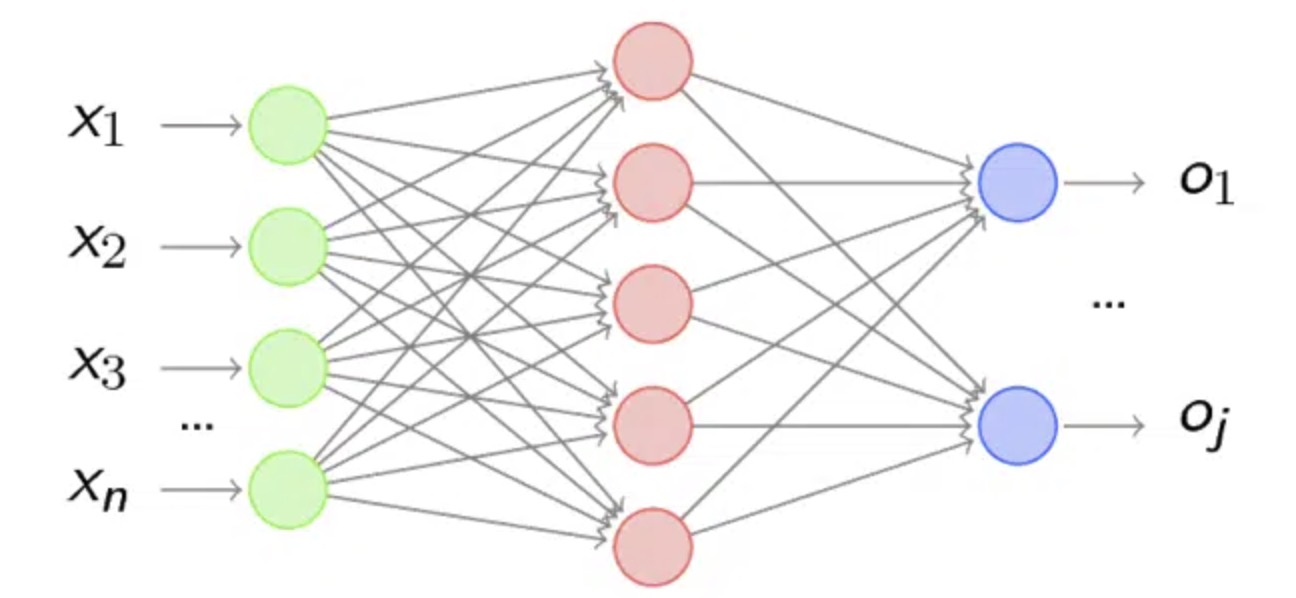
\includegraphics[scale=0.2]{7.jpeg}
    \caption{卷积层实现}
    \label{figure}
 \end{figure}

\section{研究所用到的神经网络模型}

\subsection{VGG16}
VGG16是牛津大学的K.Simonyan和A.Zisserman在论文“Very Deep Convolutional Networks for Large-Scale Image Recognition”中提出的卷积神经网络模型。 

其网络结构具有一定的规律性。该网络接受224×224的RGB图像作为输入,经过一系列的卷积层和最大池化层,输出一个1000维的向量,表示图像的类别概率。

VGG16网络包含13个卷积层和3个全连接层,其中卷积层都采用3×3的卷积核进行特征提取,并使用ReLU激活函数进行非线性变换。卷积层之后的最大池化层通过对特征图进行下采样,提取最显著的特征。

在网络的末尾,VGG16采用三个全连接层进行分类。前两个全连接层各自有4096个神经元,最后一个全连接层有1000个神经元,每个神经元对应于一个类别。最后一层是softmax层,将输出向量转化为类别概率。

VGG16结构如下:
\begin{figure}[H]
    \centering
    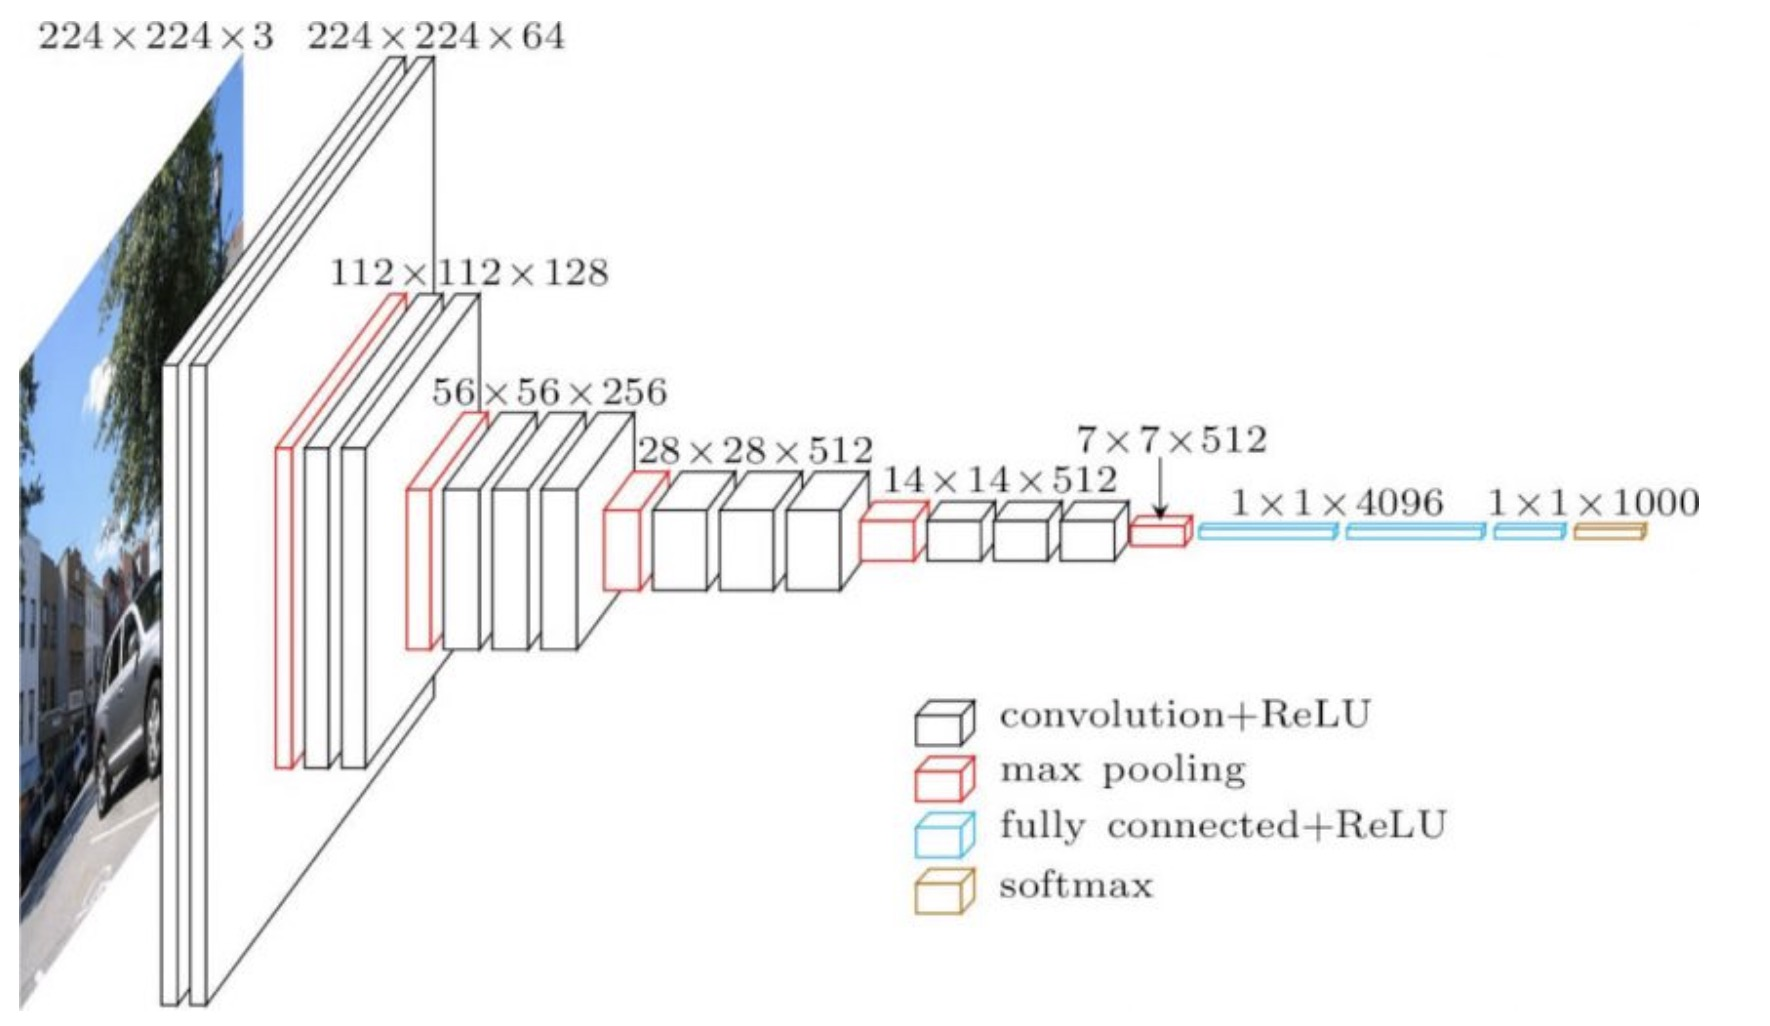
\includegraphics[scale=0.2]{8.jpeg}
    \caption{VGG16}
    \label{figure}
 \end{figure}

\subsection{ResNet50}
ResNet50是一个经典的深度卷积神经网络,由何凯明等人于2015年提出,是ResNet系列中较为流行的一个网络结构。
ResNet50共包含50个卷积层,其中包括16个Bottleneck块和一个全局平均池化层,最后连接一个具有1000个输出的全连接层,
用于ImageNet分类任务。

ResNet50引入了残差学习的思想,通过在网络中加入残差块来缓解梯度消失问题。
每个残差块包含两个3x3卷积层和一个跨层连接,其中跨层连接绕过了一个或多个卷积层,将输入直接添加到输出上。
这种跨层连接方式使得模型可以更好地捕捉到输入特征的变化,同时避免了梯度消失的问题,使得网络训练更加容易。

\begin{figure}[H]
    \centering
    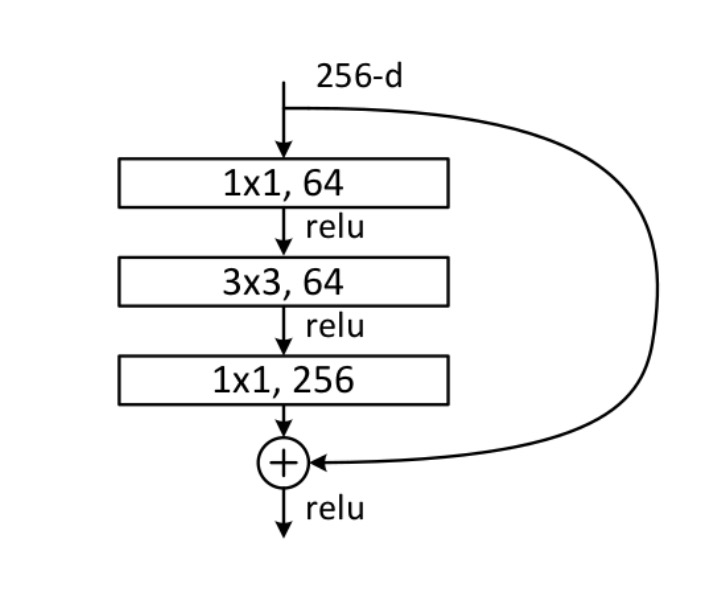
\includegraphics[scale=0.2]{10.jpeg}
    \caption{VGG16}
    \label{figure}
 \end{figure}

ResNet50在许多计算机视觉任务中都表现出色,
不仅在ImageNet分类任务中取得了优异的成绩,同时在物体检测、语义分割等任务中也广泛应用。
同时,ResNet50也为后来的深度神经网络提供了很多启示,如更深层次的ResNet-101、ResNet-152等。

\subsection{DenseNet201}
DenseNet201是一种深度卷积神经网络,是2016年由Kaiming He等人提出的。
它的主要特点是密集连接(Dense Connectivity),即每个层的输出都与之前所有层的输出连接在一起,形成了一个密集的连接结构,这样可以有效地提高特征复用和梯度流动,
使得模型的性能得到了大幅度的提升。

DenseNet201的网络结构相对较深,包含多个密集块(Dense Block),每个密集块内部由多个卷积层、BN层和ReLU激活层构成。
在每个密集块的末尾,还包含了一个转换层(Transition Layer),用于控制特征图的尺寸和通道数。整个网络还包含了一个全局平均池化层和一个softmax分类器。

DenseNet201在多个计算机视觉领域的任务中都表现出了很好的性能,比如图像分类、目标检测、语义分割等。同时,由于它的密集连接结构,它在参数数量和计算复杂度方面也有一定的优势。因此,DenseNet201是一种非常有用的深度学习模型。


\section{算法流程}

算法主要流程如下:

1.导入所需的Python库。

2.从图像目录中加载图像并将它们转换为数组。

3.为良性和恶性样本创建标签,合并数据并将其打乱。

4.将标签转换为分类矩阵。

5.创建卷积神经网络模型。并使用生成器对模型进行训练,设置回调函数以在验证集上监控模型的性能并定期保存最模型。

6.在验证集上进行预测并评估模型性能。

\chapter{实验和分析}
\section{数据集}
\subsection{BreakHis数据集}
乳腺癌组织病理学图像数据集BreaKHis,收集自82位患者的乳腺肿瘤组织样本,共包含9,109幅显微图像,分别使用不同放大倍数
(40X、100X、200X和400X)获得。该数据集目前已包含2,480个良性样本和5,429个恶性样本,图像大小为700×460像素,以3通道RGB格式存储,每个通道有8位深度,采用PNG格式保存。

总体而言,BreaKHis数据集可分为两个主要类别:良性肿瘤和恶性肿瘤。
组织学良性指的是不符合任何恶性标准的病变,例如,细胞形态正常、无明显的有丝分裂、基底膜未破裂和未发生转移等。
通常,良性肿瘤的生长缓慢、范围有限,相对较为“温和”。
恶性肿瘤是癌症的同义词,该病变可侵犯并破坏周围的结构(局部浸润),并向远处扩散(转移),最终导致患者死亡。

BreakHis数据集结构如下:


\begin{table}[H]
    \centering
    \caption{BreakHis数据集结构}
    \begin{tabular}{|c|c|c|c|} % 控制表格的格式,可以是l,c,r
    \hline
    Magnification & Benign & Malignant & Total\\
    \hline
    40X & 652 & 1,370 & 1,995\\
    \hline
    100X & 644 & 1,437 & 2,081\\
    \hline
    200X & 623 & 1,390 & 2,013\\
    \hline
    400X & 588 & 1,232 & 1,820\\
    \hline
    Total of Images & 2,480 & 5,429 & 7,909\\
    \hline
    \end{tabular}
    \label{tbl_mos1_nanotube}



\end{table}
下面是BreakHis数据集中的一些图片:
\begin{figure}[H]
    \centering
    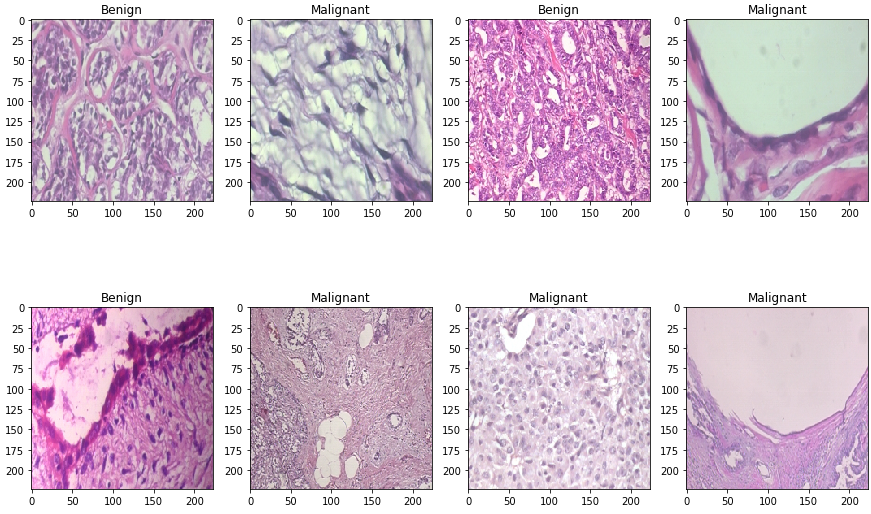
\includegraphics[scale=0.2]{14.png}
    \caption{BreakHis}
    \label{figure}
 \end{figure}


\subsection{INbreast数据集}
INbreast是一个用于数字乳腺X射线图像识别和分割的公共数据集,其中包含了410张数字乳腺X射线图像和对应的乳腺组织分割掩模。
这个数据集可以用于乳腺癌筛查和诊断等医学研究领域。该数据集中的图像是由印度国立癌症研究所的专业医生进行标注和诊断的。

INbreast数据集中的每张乳腺X射线图像都包含了医生的诊断结果,包括该乳腺病变是否为恶性(乳腺癌)等信息。
该数据集中的图像被标记为“良性”或“恶性”,并且每个标注都由两名专业医生进行独立审核和诊断,以确保标注的准确性和可靠性。
同时,数据集中也包含了一些异常和其他诊断结果的标注,例如乳腺增生和钙化等。这些诊断结果和标注信息可以帮助研究人员进行乳腺癌筛查和诊断算法的开发和评估。

INbreast数据集中的每张图像的标注信息可以通过查看相应的XML文件来获取。
每个XML文件都与该图像的文件名相对应,并且包含了该图像的详细标注信息,例如病变的位置、大小、形状、密度等等

部分信息如下:
\begin{figure}[H]
    \centering
    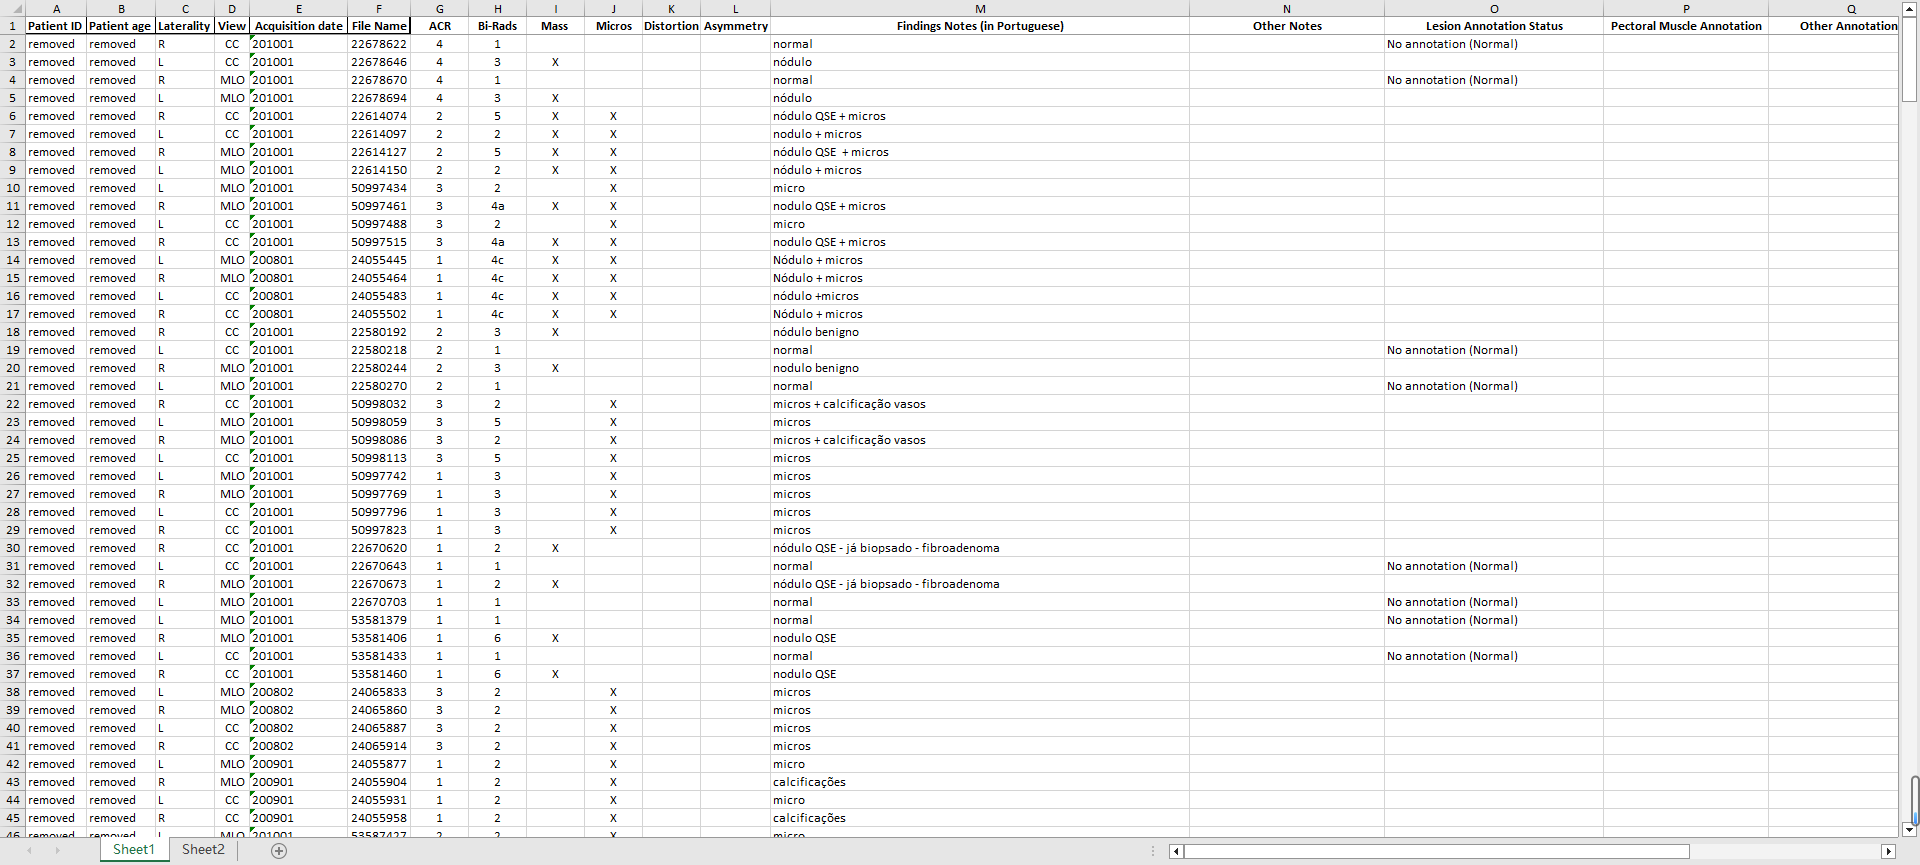
\includegraphics[scale=0.2]{15.png}
    \caption{BreakHis}
    \label{figure}
 \end{figure}
  
 由于该表格只是给出了相关的指标和诊断建议,并没有具体的良性恶性标签。所以在实际实验中根据表中的Bi-Ras值对图片进行标记。
 它是用于乳腺X线摄影检查结果分类的一种标准,包括0-6级,用于评估乳房肿块或其他异常发现的可能性。这些级别包括:

 0级:需要进一步影像学检查和/或额外的评估。

 1级:阴性,无明显异常。

 2级:良性,无恶性病变的病理学特征。

 3级:概率良性,但建议进行短期随访检查。

 4级:可疑,建议进行进一步组织学检查。

 5级:高度可疑,建议进行活检。

 6级:已知为恶性病变,需进行治疗。


 在实际打标签的过程中,将0-3标记为良性而将4-6标记为恶性。

 

\section{实验结果分析}
\subsection{不同的数据集结构}
首先在选用BreakHis数据集进行二分类时,整个数据集进行如下分割:
\begin{figure}[H]
    \centering
    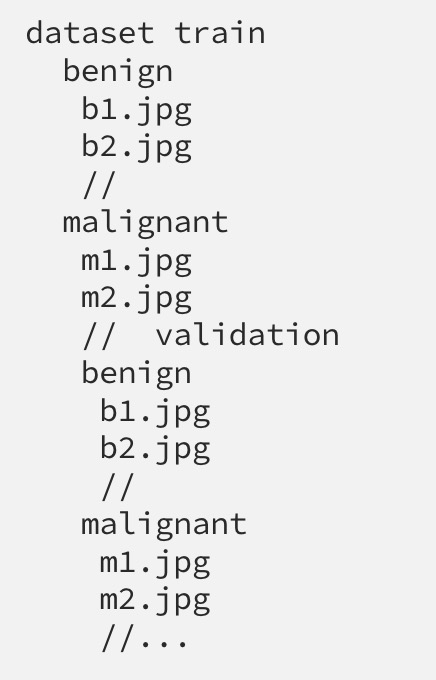
\includegraphics[scale=0.2]{11.jpeg}
    \caption{4分类+4分类}
    \label{figure}
 \end{figure}

由于数据集中良性与恶性的样本数量不匹配,以以下两种方法进行实验。
一种是使用原始的数据集,即将测试集和训练集中包含整个数据集中的所有样本。二是对整个数据集进行抽取,使得良性和恶性
样本的数量相匹配。具体抽取规则为训练集良性与恶性每个类别各有 1000 张图像,而验证文件夹每个类别各有 250 张图像。

\begin{figure}[H]
    \centering
    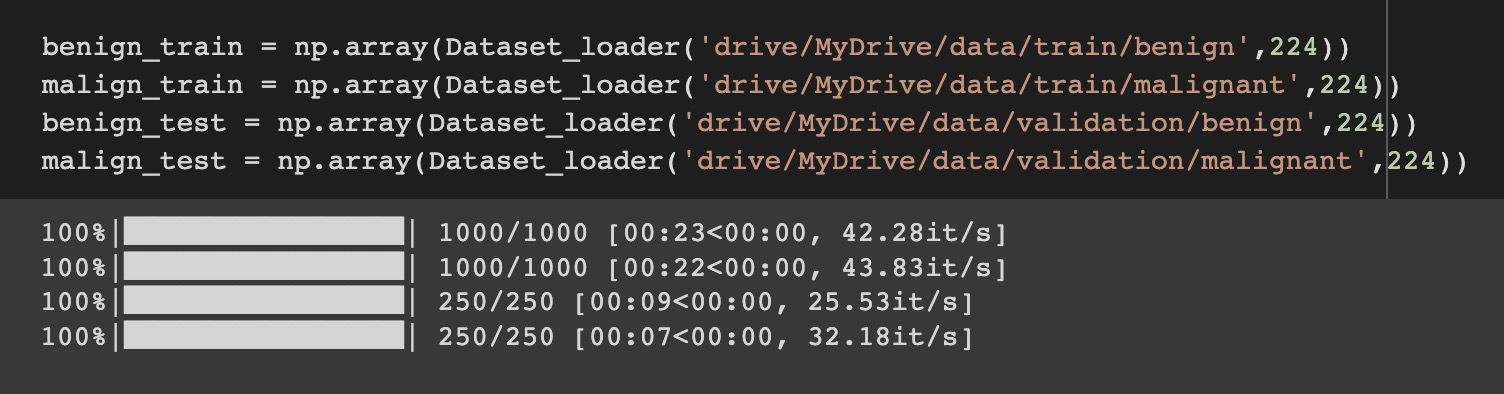
\includegraphics[scale=0.2]{12.jpeg}
    \caption{抽取后的数据集}
    \label{figure}
 \end{figure}


 \begin{figure}[H]
    \centering
    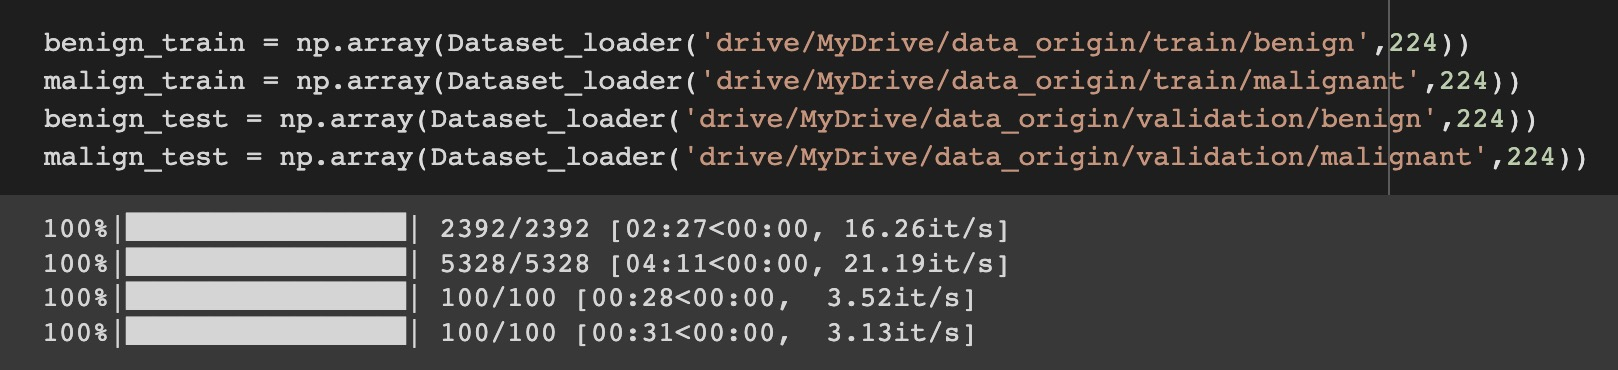
\includegraphics[scale=0.2]{13.jpeg}
    \caption{原数据集}
    \label{figure}
 \end{figure}

通过实验,经过抽取后的


\subsection{不同的分类方式}
而根据肿瘤细胞在显微镜下的外观,又可以将良性和恶性乳腺肿瘤分为不同的类型。
各种类型/亚型的乳腺肿瘤可能具有不同的诊断和治疗意义。
该数据集目前包含四种不同组织学类型的良性乳腺肿瘤:腺病 (A)、纤维腺瘤 (F)、叶状肿瘤 (PT) 和管状腺酮 (TA);
和四种恶性肿瘤(乳腺癌):癌(DC)、小叶癌(LC)、粘液癌(MC)和乳头状癌(PC)。
 
据此在本文在实现乳腺癌图像分类时采用了不同的分类标准,并对结果进行了比较。一是最基础的二分类,即将所有图像仅分成良性
恶性两类。

\begin{figure}[H]
    \centering
    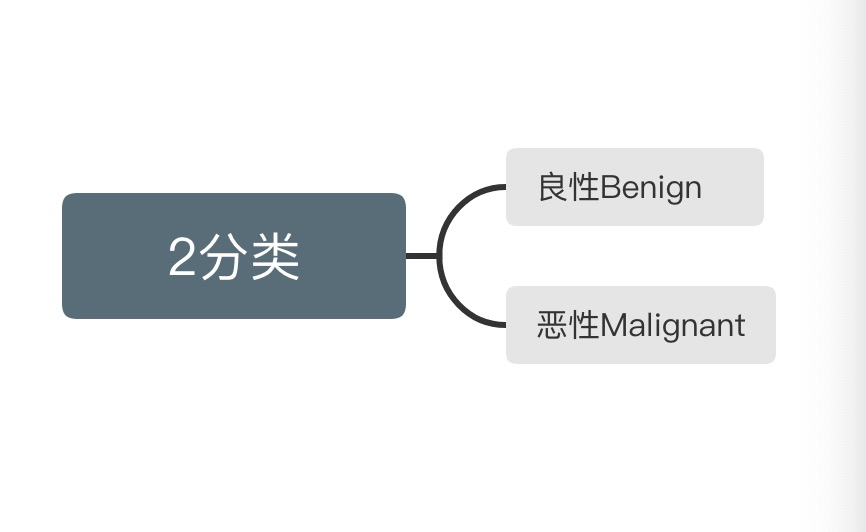
\includegraphics[scale=0.2]{1.jpeg}
    \caption{2分类}
    \label{figure}
 \end{figure}


二是直接进行8分类,即直接将整个数据集分成A,F,PT,TA,DC,LC,MC,PC8类。

\begin{figure}[H]
    \centering
    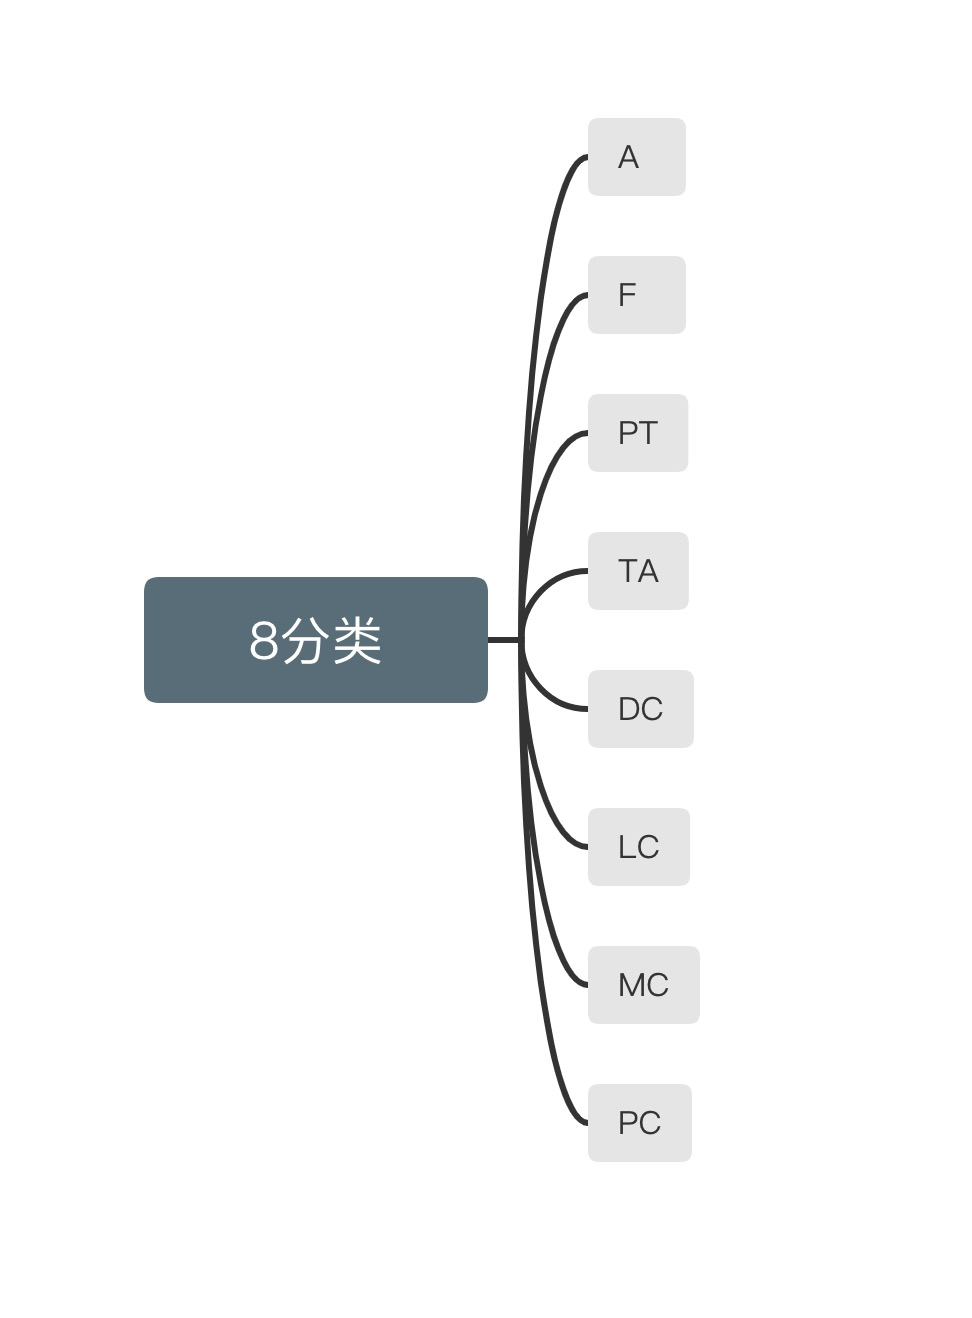
\includegraphics[scale=0.2]{2.jpeg}
    \caption{8分类}
    \label{figure}
 \end{figure}


三是分别对良性和恶性两个数据集进行四分类。

\begin{figure}[H]
    \centering
    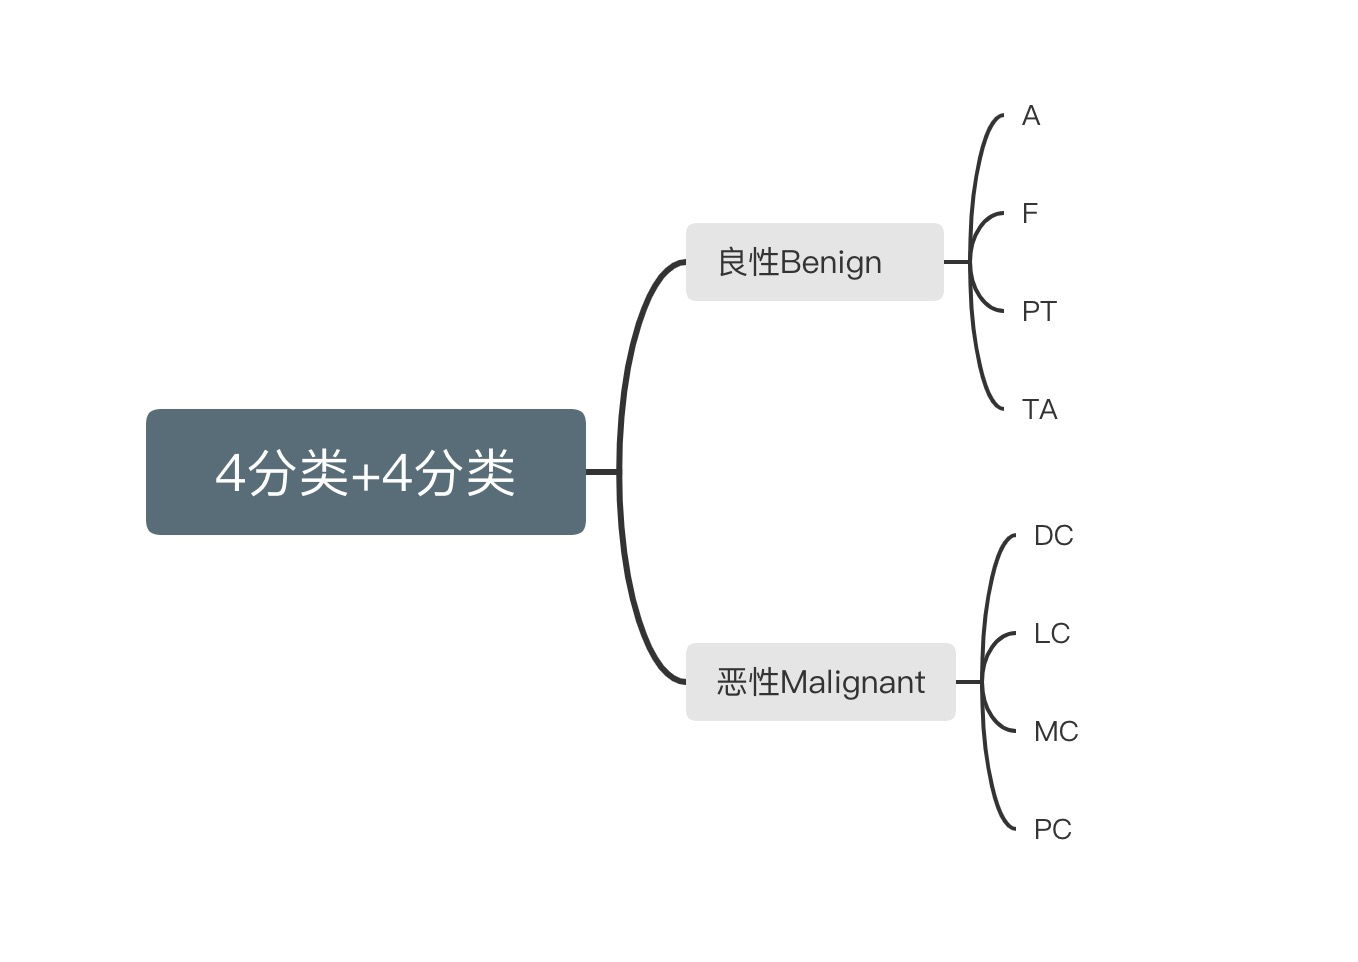
\includegraphics[scale=0.1]{3.jpeg}
    \caption{4分类+4分类}
    \label{figure}
 \end{figure}

 

\subsection{不同的神经网络模型}


\subsection{不同的数据集}



\subsection{附页代码} % (fold)
\label{sub:附页代码}
可以在LZUThesis.clc里面修改代码格式

java代码
\begin{lstlisting}[language = java]
    System.out.print("兰朵儿")
    // 试一下中文注释
\end{lstlisting}


tex代码
\begin{lstlisting}[language = tex]
    width=0.3\textwidth
    % 注释
\end{lstlisting}

python代码
\begin{lstlisting}[language = python]
    print("兰朵儿")
    # 注释
\end{lstlisting}

matlab代码有专门的库,但是没必要高亮太多,而且中文适配有问题,直接按照下面这个就可以
\begin{lstlisting}[language = matlab]
    display("兰朵儿")
    % 注释
\end{lstlisting}

% subsection 附页代码 (end)

伪代码

\begin{algorithm}[H]
    \caption{PMHSS 算法\label{Alg:PMHSS}}
    \begin{algorithmic}[1]
      \State 给定一个初值 $ x^{(0)} \in C^{n} $  和常数 $\alpha>0$
      \For{$k = 1,2, \ldots $ 直到序列 $\{x^{(k)}\}_{k=0}^{\infty}$ 收敛}
      \State 解方程: $(\alpha V+W)x^{(k+\frac{1}{2})}=(\alpha V-i T)x^{(k)}+b $
      \State 解方程: $(\alpha V+T)x^{(k+1)}=(\alpha V+i W)x^{(k+\frac{1}{2})}-i b$
      \EndFor
    \end{algorithmic}
\end{algorithm}

\subsection{参考文献} % (fold)
\label{sub:参考文献}

这个,百度学术、谷歌学术等网站都可以导出bibtex格式的参考文献(知网不行,网上有个人写了个转换器,但是windows用不了,就不放了,尽量用谷歌学术把那个文献找出来吧),直接放在bib/database.bib文件里、知网需要用其他东西转换,但是我建议用mendeley这个软件管理文献,然后可以导出bibtex格式的,甚至可以直接复制引用,很方便\cite{partl2016, tenne1992polyhedral, tussyadiah2015hotels}。

有些人希望多个参考文献同时引用时用[1-3]而不是[1,2,3],所以我加了个包cite。(2020-5-18)

具体怎么用可以百度,我这里告诉你什么可以用,但是具体的,建议百度,更靠谱一些。


有参考文献时,编译要经过4步,直接XeLaTeX --> BibTeX --> XeLaTeX --> XeLaTeX,不然很多问题,vscode配置以后很方便,以下内容放在设置中,重新打开vscode即可

修改后可以参考文献自动生成中文等字符\cite{partl2021}\cite{partl2022}\cite{partl2022-2},引用网络资源时链接格式规范化\cite{intelnewsroomIntelUnveils12th2021,wilsonHistoryDevelopmentParallel1994}。

测试右上角 \upcite{partl2021}

\subsubsection{中英文参考文献说明} % (fold)

感谢的代码贡献
\href{https://gitee.com/versemonger}{潘麒}

进一步说明,对于中文参考文献,建议添加条目 language={中文} 这一行,否则多个作者,不是 “等.”\cite{partl2021} 而是 “et al.”\cite{partl2016}
\begin{lstlisting}[language = tex]

    @Article{partl2021,
    author = {Partl, Hubert and Hyna, Irene  and 兰朵儿 and Schlegl, Elisabeth},
    title  = {一个中文等测试},
    year   = {2021},
    language = {中文},
    journal = {测试期刊},
    volume={3},
    number={6},
    pages={10--20},
  }
  
\end{lstlisting}


% subsection 参考文献 (end)

% section 图标等常用的教程 (end)

\subsection{引用图、表、公式、章节} % (fold)

为什么要引用?不直接写数字?因为图表顺序变化时,引用的地方会自动变化。每次更加新引用,请四步走编译

引用的地方加label,自己写个名字,可以是中文,然后引用的地方如下:

如图\ref{fig_ldr}所示

如公式\eqref{e1e2}所示,会自动带括号

如表\ref{tbl_gs}所示

在\ref{sub:参考文献}中已经提及


%论文后部
\backmatter


%=======%
%引入参考文献文件
%=======%
\bibdatabase{bib/database}%bib文件名称 仅修改bib/ 后部分
\printbib
% \nocite{*} %显示数据库中有的,但是正文没有引用的文献



\Appendix


这里是附录页,附上你的程序或必要的相关知识

{\bfseries 编译方式:} XeLaTeX -->BibTeX --> XeLaTeX-->XeLaTeX


\Thanks

这里是致谢页,你可以在这里致谢你的舍友,老师,朋友,或者我

(我是谁?兰朵儿开发者:余航,致谢我,查重时一定会重复的,哈哈,开个玩笑,本科生论文不在查重范围,而且“毕业论文(设计)检测内容主要为毕业论文(设计)的主体部分”)。


\Grade %这一句才是成绩页,上面是填写


\end{document}
